\section{Autoencoders}

\begin{frame}{We Interrupt Your Regularly Scheduled Programming\dots}

\begin{columns}
\begin{column}{0.1\textwidth}
\end{column}
{%
\setlength{\fboxrule}{3pt}
\fcolorbox{lightgray}{extralightgray}{
\begin{column}{0.8\textwidth}
\centering
\begin{minipage}{0.9\textwidth}
\raggedright
\Large
\vspace{2ex}
The paper seems to be about autoencoders, not evolutionary algorithms.
\vskip5mm
\raggedleft
\large
--- Reviewer \#4\\
\vspace{2ex}
\end{minipage}

\end{column}
}
}
\begin{column}{0.1\textwidth}
\end{column}
\end{columns}

\end{frame}
\begin{frame}{We Interrupt Your Regularly Scheduled Programming\dots}

\begin{columns}
\begin{column}{0.1\textwidth}
\end{column}
{%
\setlength{\fboxrule}{3pt}
\fcolorbox{lightgray}{extralightgray}{
\begin{column}{0.8\textwidth}
\centering
\begin{minipage}{0.9\textwidth}
\raggedright
\Large
\vspace{2ex}
We'll use autoencoders to do cool evolution things, I promise!
\vskip5mm
\raggedleft
\large
--- me\\
\vspace{2ex}
\end{minipage}

\end{column}
}
}
\begin{column}{0.1\textwidth}
\end{column}
\end{columns}

\end{frame}

\begin{frame}{Autoencoder Intuition}

\vspace{1ex}
{\Large
\textbf{What does an autoencoder do?}%
\only<5>{%
\footnote{not just for faces!}
}
}%

\vspace{1ex}

\begin{figure}


\begin{columns}
\begin{column}{0.4\textwidth}
\onslide<2->{
\includegraphics[width=\textwidth]{guy}
}
\end{column}
\begin{column}{0.2\textwidth}
\onslide<3->{
\centering
\Large
auto encoder\\[1ex]

\includegraphics[width=\textwidth]{arrow}
}
\end{column}
\begin{column}{0.4\textwidth}
\onslide<4->{
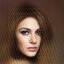
\includegraphics[width=\textwidth]{curly-guy/latent-6}
}
\end{column}
\end{columns}
\vspace{1ex}

\begin{columns}
\begin{column}{0.4\textwidth}
\onslide<2->{
\Large
\centering
input
}
\end{column}
\begin{column}{0.2\textwidth}
\end{column}
\begin{column}{0.4\textwidth}
\onslide<4->{
\Large
\centering
reconstructed input
}
\end{column}
\end{columns}

\vspace{1ex}
\onslide<2->{
\caption{
Autoencoders take an input and then return a reconstructed input.
Graphics from \cite{white2016sampling}.
}
}
\end{figure}
\vspace{-3ex}
\end{frame}

\begin{frame}{Autoencoder Intuition}

{\Large
\textbf{Why are autoencoders useful?}
}

\pause

\vspace{4ex}

{\Large
two superpowers:

\pause

\begin{enumerate}

\item compression \onslide<5->{\textcolor{h2}{$\leftarrow$ bottlenecked autoencoder}}

\pause

\item de-corruption \onslide<6>{\textcolor{h2}{$\leftarrow$ denoising autoencoder}}

\end{enumerate}
}

\end{frame}

\begin{frame}{Autoencoder Intuition: Bottlenecked}

\begin{figure}

  \centering

  \begin{columns}
  \begin{column}{0.25\textwidth}
  \Large
  \centering
  \phantom{input}
  \includegraphics[width=\textwidth]{img/guy}\\
  input
  \end{column}
  \begin{column}{0.5\textwidth}
  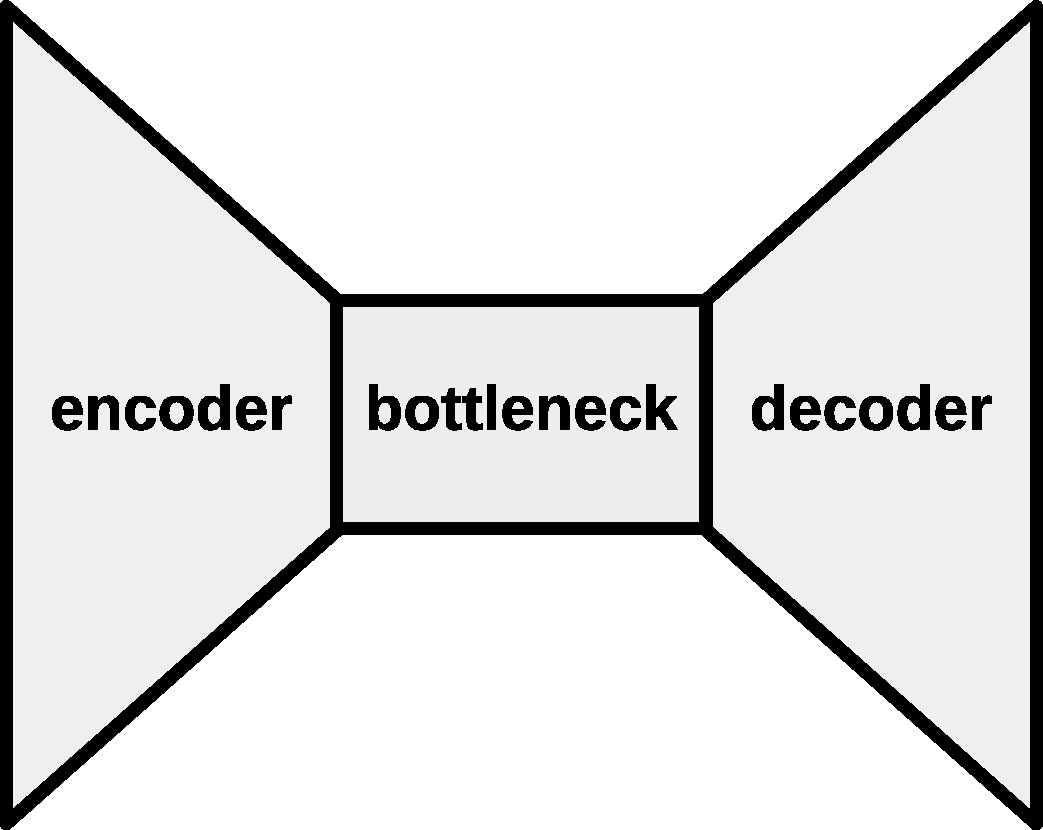
\includegraphics[width=\textwidth]{img/stripped_bottleneck}
  \end{column}
  \begin{column}{0.25\textwidth}
  \Large
  \centering
  ~\\[1.35ex]
  \phantom{input}
  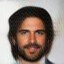
\includegraphics[width=\textwidth]{img/curly-guy/latent-6}\\
  reconst \\ input
  \end{column}
  \end{columns}

  \vspace*{-9.35ex}

  \makebox(0,0){
    
\includegraphics[width=0.1\textwidth]{static/static-1}\hspace{0.075ex}
  }

  \vspace*{9.35ex}


  \caption{
  Summary of bottlenecked autoencoders, which generate a compact encoding  (greyscale matrix) of a particular class of input (e.g., faces) then reconstruct the presented input.
  Graphics from \cite{white2016sampling}.
  }
\end{figure}

\end{frame}

\begin{frame}{Autoencoder Intuition: Bottlenecked}

\begin{figure}

  \begin{columns}
  \begin{column}{0.07\textwidth}
  \end{column}
  \begin{column}{0.6\textwidth}
  \small
  \centering
  \begin{columns}
  \begin{column}{0.225\textwidth}
  \centering
  input
  \end{column}
  \begin{column}{0.2\textwidth}
  \centering
  encoder
  \end{column}
  \begin{column}{0.15\textwidth}
  \centering
  bottle neck
  \end{column}
  \begin{column}{0.2\textwidth}
  \centering
  decoder
  \end{column}
  \begin{column}{0.225\textwidth}
  \centering
  reconst input
  \end{column}
  \end{columns}

  \vspace{1ex}

  \begin{columns}
  \begin{column}{0.225\textwidth}
  \centering
  \includegraphics[width=\textwidth]{guy}
  \end{column}
  \begin{column}{0.2\textwidth}
  \centering
  
\includegraphics[width=0.75\textwidth]{arrow}
  \end{column}
  \begin{column}{0.15\textwidth}
  \centering
  
\includegraphics[width=\textwidth]{static/static-1}
  \end{column}
  \begin{column}{0.2\textwidth}
  \centering
  
\includegraphics[width=0.75\textwidth]{arrow}
  \end{column}
  \begin{column}{0.225\textwidth}
  \centering
  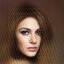
\includegraphics[width=\textwidth]{curly-guy/latent-6}
  \end{column}
  \end{columns}

  \vspace*{1.5ex}

  \makebox(0,0){
    $\bm{\vdots}$
  }

  \vspace*{3.25ex}

  \begin{columns}
  \begin{column}{0.225\textwidth}
  \end{column}
  \begin{column}{0.2\textwidth}
  \end{column}
  \begin{column}{0.15\textwidth}
  \centering
  
\includegraphics[width=\textwidth]{static/static-2}
  \end{column}
  \begin{column}{0.2\textwidth}
  \centering
  
\includegraphics[width=0.75\textwidth]{arrow}
  \end{column}
  \begin{column}{0.225\textwidth}
  \centering
  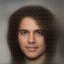
\includegraphics[width=\textwidth]{curly-guy/latent-3}
  \end{column}
  \end{columns}

  \vspace*{1.5ex}

  \makebox(0,0){
    $\bm{\vdots}$
  }

  \vspace*{3.25ex}

  \begin{columns}
  \begin{column}{0.225\textwidth}
  \centering
  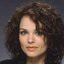
\includegraphics[width=\textwidth]{curly}
  \end{column}
  \begin{column}{0.2\textwidth}
  \centering
  
\includegraphics[width=0.75\textwidth]{arrow}
  \end{column}
  \begin{column}{0.15\textwidth}
  
\includegraphics[width=\textwidth]{static/static-3}
  \end{column}
  \begin{column}{0.2\textwidth}
  \centering
  
\includegraphics[width=0.75\textwidth]{arrow}
  \end{column}
  \begin{column}{0.225\textwidth}
  \centering
  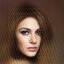
\includegraphics[width=\textwidth]{curly-guy/latent-1}
  \end{column}
  \end{columns}

  \end{column}
  \begin{column}{0.03\textwidth}
  \end{column}
  \begin{column}{0.3\textwidth}
  \caption{
  ~\\
  Summary of latent space interpolation.
  Intermediate bottlenecked encodings between two input images are visualized.
  Graphics from \cite{white2016sampling}.
  }
  \end{column}
  \end{columns}

\end{figure}

\end{frame}

\begin{frame}{Autoencoder Intuition: Bottlenecked}

\begin{figure}

\begin{columns}
\begin{column}{0.6\textwidth}
\foreach \n in {1,...,12}{%
\includegraphics<\n>[width=\textwidth]{latent-walk/latent-\n}%
}%
\end{column}
\begin{column}{0.4\textwidth}
\caption{
Frame-by-frame latent space interpolation animation.
Graphics from \cite{white2016sampling}.
}
\end{column}
\end{columns}

\end{figure}

\end{frame}


\begin{frame}{Autoencoder Intuition: Denoising}

\begin{figure}

\begin{columns}
\begin{column}{0.3\textwidth}
\includegraphics<1>[width=\textwidth]{reconstruct/original-senior}
\includegraphics<2->[width=\textwidth]{reconstruct/corrupted-senior}
\end{column}
\begin{column}{0.4\textwidth}
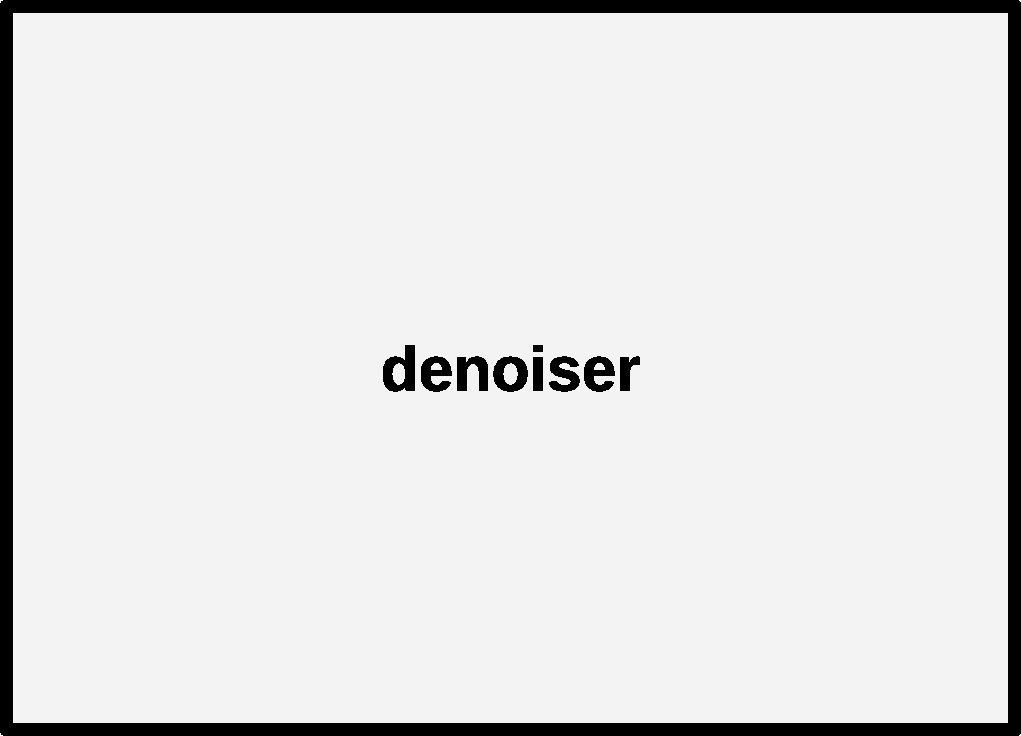
\includegraphics[width=\textwidth]{stripped_denoiser}
\end{column}
\begin{column}{0.3\textwidth}
\includegraphics[width=\textwidth]<3->{reconstruct/reconstructed-senior}
\end{column}
\end{columns}

\vspace{1ex}

\begin{columns}
\begin{column}{0.3\textwidth}
\centering
\only<1>{input}
\only<2->{corrupted input}
\end{column}
\begin{column}{0.4\textwidth}
\end{column}
\begin{column}{0.3\textwidth}
\centering
\only<1,2>{\phantom{reconst input}}
\only<3->{reconst input}
\end{column}
\end{columns}

\vspace{1ex}

\caption{
Summary of denoising autoencoder, which receives a corrupted copy of a particular class of input (e.g., faces) and attempts to recover the uncorrupted input.
Graphics from \cite{allen2018generative}.
}
\end{figure}

\end{frame}


\begin{frame}{Autoencoder Implementation}

\Large

\textbf{What's under the hood?}

\pause

\vspace{3ex}
\centering

\HUGE
\onslide<3->{%
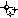
\includegraphics[width=1em]{emoji-star}%
}%
~deep learning
\onslide<3->{%
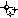
\includegraphics[width=1em]{emoji-star}%
}

\normalsize
\onslide<4->{
(a.k.a. big artificial neural networks + big training data)
}

\end{frame}

\begin{frame}{Autoencoder Implementation: Training}
\begin{figure}
\includegraphics[width=0.8\textwidth]{celeba}
\caption{
Training requires a large, representative set of examples of the class of objects to autoencode.
Graphic from \cite{liu2015faceattributes}.
}
\end{figure}
\end{frame}
